\documentclass{beamer}
\usepackage{listings}
\usepackage{booktabs}
\usepackage{bookmark}
\usepackage{makecell}
\usepackage{amsmath}
\usepackage{url}
\usepackage{multirow}
\usepackage{graphicx}


\usepackage{beamerthemesplit}
\usetheme{Berkeley}

\definecolor{colorgreen}{rgb}{0,0.6,0}
\definecolor{colorgray}{rgb}{0.5,0.5,0.5}
\definecolor{colorpurple}{rgb}{0.58,0,0.82}
\definecolor{colorback}{RGB}{255,255,204}
%Definiendo el estilo de las porciones de codigo
\lstset{
 backgroundcolor=\color{colorback},
commentstyle=\color{colorgreen},
keywordstyle=\color{colorpurple},
numberstyle=\tiny\color{colorgray},
stringstyle=\color{colorpurple},
basicstyle=\ttfamily\footnotesize,
breakatwhitespace=false,
breaklines=true,
captionpos=b,
keepspaces=true,
numbers=left,
showspaces=false,
showstringspaces=false,
showtabs=false,
tabsize=2,
frame=single,
framesep=2pt,
rulecolor=\color{black},
framerule=1pt
}

\title{Moogle!}
\subtitle{}
\institute{Facultad de Matemática y Computación\\Universidad de la Habana}
\author{Richard Alejandro Matos Arderí}
\date{2023}


\begin{document}
\maketitle

\begin{frame}
\tableofcontents
\end{frame}

\section{¿Qué es Moogle! y cómo usarlo?}

\begin{frame}
\begin{figure}[h]
       \center
       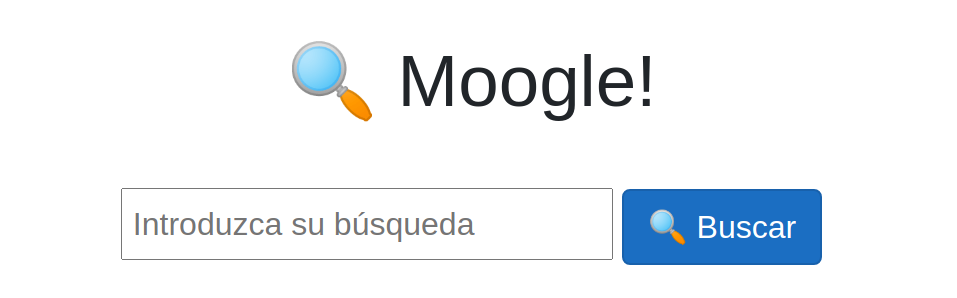
\includegraphics[width=8cm]{Web2.jpg}
\end{figure}
Moogle! es una aplicación cuyo propósito es buscar inteligentemente un texto en
un conjunto de documentos. Es una aplicación web, desarrollada con tecnología .NET
Core 6.0, específicamente usando Blazor como *framework* web para la interfaz
gráfica, y en el lenguaje C\#.
\end{frame}
\begin{frame}{¿Cómo funciona?}
Moogle! utiliza los conceptos de TF-IDF para asignar a cada uno de los documentos .txt sobre los que opera, un vector, que mediante el algoritmo de similitud por coseno es comparado con el vector generado a partir de la entrada del usuario. Además de devolver los títulos de los documentos organizados de acuerdo a la relevancia que tengan en relación con la búsqueda realizada , Moogle! contiene otras funcionalidades que enriquecen la interacción. De conjunto con cada título está un fragmento del mismo que contiene la porción de la entrada más significativa de acuerdo con su valor TF-IDF y en caso de que alguna de las palabras de la entrada no exista en ningún documento se devolverá como sugerencia el texto contenido en la colección de documentos con mayor similitud a la entrada del usuario utilizando el algoritmo de la distancia de Levenshtein.
\end{frame}


\subsection{Modo de uso}
\begin{frame}

Siga las siguientes instrucciones:
\begin{enumerate}
\item Ingrese palabras clave relacionadas con la información que desea encontrar en el campo de búsqueda.
\item Haga clic en "Buscar" para obtener una lista de resultados relevantes.
\item Explore los resultados y obtenga una vista previa de los fragmentos de texto relevantes.
\item Si alguna palabra clave no arroja resultados, Moogle ofrecerá una  sugerencia de búsqueda similar.
\item Explore más resultados o realice nuevas búsquedas según sea necesario.
\end{enumerate}



\end{frame}
\begin{frame}{Ejemplo de Sugerencia}
\begin{figure}[h]
       \center
       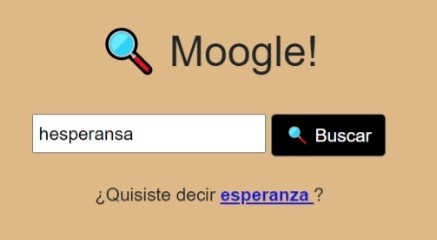
\includegraphics[width=8cm]{Web3.jpg}
\end{figure}
\end{frame}

\section{Base del modelo vectorial}
\begin{frame}
Fueron implementados los siguientes conceptos para el proceso de organización de resultados de la búsqueda:
\begin{itemize}
\item TF-IDF
\item Similitud por coseno
\item Distancia de Levenshtein
\end{itemize}
\end{frame}

\subsection{TF-IDF}
\begin{frame}{Fórmula de TF-IDF}
\[TF-IDF = \frac{Xi}{Ni} \times ln\left(\frac{D}{P}\right)\]
Donde:
\begin{itemize}
\item $Xi$
representa la frecuencia absoluta de una palabra en un documento.
\item $Ni$
representa la cantidad de palabras del documento en cuestión.
\item $D$
representa la cardinalidad de la colección de documentos.
\item $P$
representa la cantidad de documentos en los que aparece la palabra.
\end{itemize}

\end{frame}
\subsection{Similitud por coseno}
\begin{frame}{Producto Punto y Magnitud de un vector}
\begin{enumerate}
\item Cálculo del producto punto:
\begin{itemize}
 \item  El producto punto se calcula multiplicando las correspondientes componentes de los vectores y sumándolos. Por ejemplo, el producto punto entre los vectores [2, 1, 0, 3] y [1, 0, 1, 2] sería: \[(2\times 1) + (1\times 0) + (0\times 1) + (3\times 2) = 8\].
\end{itemize}
\item  Cálculo de las magnitudes de los vectores:
\begin{itemize}
  \item  La magnitud de un vector se calcula sumando los cuadrados de sus componentes y luego tomando la raíz cuadrada del resultado.
  \item  Por ejemplo, la magnitud del vector [2, 1, 0, 3] se calcularía como:\[\sqrt{(2^2) + (1^2) + (0^2) + (3^2)} = \sqrt{4 + 1 + 0 + 9} = \sqrt{14}\].
\end{itemize}
\end{enumerate}
\end{frame}

\begin{frame}{Similitud}
Cálculo de la similitud por coseno:
\begin{itemize}
   \item La fórmula para calcular la similitud por coseno es: \[\text{similitud} = \frac{{\text{producto punto}}}{{\text{magnitud vector1} \times \text{magnitud vector2}}}\].
  \item En el ejemplo anterior, la similitud por coseno entre los vectores [2, 1, 0, 3] y [1, 0, 1, 2] sería: \[\frac{8}{{\sqrt{14} \times \sqrt{6}}} \approx 0.765\].
\end{itemize}
\end{frame}

\subsection{Distancia de Levenshtein}
\begin{frame}
La distancia de Levenshtein se calcula determinando el número mínimo de operaciones requeridas para transformar una cadena en otra. Las operaciones permitidas son:
\begin{enumerate}

\item Inserción: Insertar un carácter en una cadena.
\item Eliminación: Eliminar un carácter de una cadena.
\item Sustitución: Reemplazar un carácter de una cadena por otro.
\end{enumerate}
Cada una de estas operaciones tiene un costo unitario asociado. La distancia de Levenshtein es la suma de los costos de todas las operaciones necesarias para transformar una cadena en la otra.
\end{frame}

\section{Estructura del proyecto}
\begin{frame}{Estructura}
La aplicación está estructurada en dos partes fundamentales: \textcolor{blue}{Moogle Server} y \textcolor{blue}{Moogle Engine}.
\end{frame}
\subsection{Moogle Server}
\begin{frame}{Moogle Server}
  \textcolor{blue}{MoogleServer} es un servidor web que renderiza la interfaz gráfica y sirve los resultados.
\end{frame}

\subsection{Moogle Engine}
\begin{frame}{Clases}
\begin{itemize}
\item Clase Coleccion
\item Clase Metodos
\item Clase Query
\item Clase Moogle
\end{itemize}
\end{frame}
\begin{frame}{Coleccion}
En esta clase se construyen todos los objetos usados para la comparación de los documentos con la entrada del usuario. Algunas de sus propiedades son:
\begin{itemize}
   \item \textcolor{red}{string[]} Archivos: Array que contiene como elementos el contenido de los archivos en string.
  \item  \textcolor{red}{string[]} Titulos: Array que contiene como elementos los títulos de los archivos en string.
  \item \textcolor{red}{List \textless string\textgreater } ListaPalabrasSinRep: Lista de palabras de toda la colección(sin repeticiones).
  \item \textcolor{red}{double[,]} TheMatrix: Matriz formada por los vectores TF-IDF de los documentos.
  \item  \textcolor{red}{Dictionary\textless string, int \textgreater} Lista: Diccionario que asocia a cada palabra presente en el documento
su frecuencia en el mismo.
\end{itemize}

\end{frame}

\begin{frame}{Clase Metodos}
La clase es asistencial, solamente contiene métodos para ser usados en la clase \textcolor{orange}{Coleccion}, encargados de leer los archivos y asistir a otros métodos.  Algunos de estos métodos son los siguientes:
\begin{itemize}

\item \textcolor{magenta}{Snipet}: Este método devuelve el string que funciona como snipet(fragmento del documento que es devuelto junto al título.
\item \textcolor{magenta}{Lector}: Este método lee el interior de cada archivo .txt y lo asigna a un valor de un array como string.
\item \textcolor{magenta}{ListaDePalabras}: Este método crea la lista de palabras que aparecem en la colección de documentos sin repeticiones.
\item \textcolor{magenta}{Similitud}: Este método calcula la similitud por coseno entre cada documento y la entrada del usuario.
\item \textcolor{magenta}{DistanciaLevenshtein}: Este método determina la distancia de Levenshtein entre dos cadenas.
\end{itemize}
\end{frame}

\begin{frame}{Clase Query}
 Su única propiedad es un array de string que contiene como términos a las palabras de la query, de ahí que para crear un objeto de este tipo es necesario pasarle como argumento un string que es precisamente la entrada del usuario.

\end{frame}

\begin{frame}{Clase Moogle}
La clase \textcolor{orange}{Moogle} contiene un método void que inicializa al objeto de tipo \textcolor{red}{Coleccion} coleccion, y dentro de su método \textcolor{magenta}{Query} de tipo \textcolor{red}{SearchResult} llama a los métodos de la clase \textcolor{orange}{Coleccion} , \textcolor{magenta}{ObtenerSearchItems} y
 \textcolor{magenta}{Sugerencia} para devolver el objeto \textcolor{red}{SearchResult}.

\end{frame}
\begin{frame}{Ejemplo de búsqueda.}
\begin{figure}[h]
       \center
       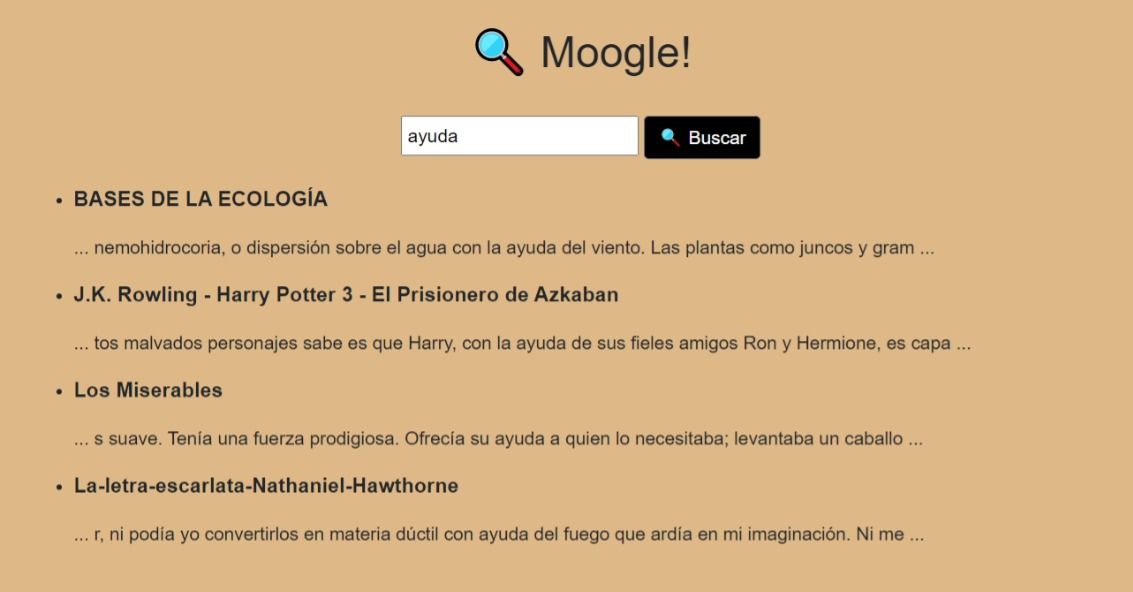
\includegraphics[width=10cm]{Web1.jpg}
\end{figure}

\end{frame}


\begin{frame}{Ejemplo de sugerencia.}
\begin{figure}[h]
       \center
       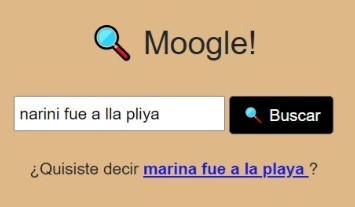
\includegraphics[width=8cm]{Web4.jpg}
\end{figure}

\end{frame}


\begin{frame}
\huge \textcolor{blue}{¡Muchas Gracias!}
\end{frame}



\end{document}
